\documentclass[a4paper,10pt]{article}

% Hier die Nummer des Blatts und Autoren angeben.
\newcommand{\blatt}{11}
\newcommand{\autor}{Ralf Engelken, Joachim Schmidberger, Frank Woithe, Michael Steinke, Merlin Koglin}

\usepackage{hci}
\usepackage{float} 

\begin{document}
% Seitenkopf mit Informationen
\kopf
\renewcommand{\figurename}{Figure}

\aufgabe{16 \textit{(Team-Aufgabe)}} 
\begin{enumerate}
\item Analyse

Im Vorfeld des Interviews hat sich der Interviewer mit der OLAT-Seite vertraut gemacht.
Dann wurde das Interview wurde mit einem OLAT-Nutzer geführt. Während des Interviews war ein PC vorhanden, auf dem die OLAT-Seite genutzt werden konnte. So konnten die Äußerungen des Interviewten direkt auf der Seite nachvollzogen werden.
Es wurde kein Fragebogen vorbereitet, die Antworten wurden schriftlich festgehalten.
\\ \\
Ergebnisse des Interviews:
\begin{enumerate}
\item{Login-Seite}

Es gibt nacheinander 2 Login-Seiten (Uni auswählen/ Benutzerlogin) von verschiedenen Servern Besser: 1 Login-Seite, keine Umleitung auf andere Server

Login Seite 1:
\begin{itemize}
\item Die Informationen für UHH und Hamburger FH sind vermischt. Besser : Trennen
\item Andere Informationen sind unübersichtlich angeordnet
\item Untermenü: Es gibt keinen Menüpunkt für den Login. Wenn man einen Menüpunkt anwählt, kommt man nicht zur Login-Seite zurück.
\item Man wird zum Login auf einen anderen Server weitergeleitet. Besser: direkter Login
\end{itemize}

Login Seite 2:
\begin{itemize}
\item Umleitung auf RRZ-Seite mit anderem Design
\item Viele unnötige Informationen (wozu Single-Signon wenn man es nur für OLAT nutzen kann?)
Besser: Seite durch direkt-Login auf der ersten Seite ersetzen
\end{itemize}


\item{Willkommen-Seite}
\begin{itemize}
\item 3 Menüebenen (horizontale Uni-Haupt-Menüleiste, vertikale Untermenüleiste, dann in Tabs aufgeteilte Seiten)
 Die Struktur ist sehr unübersichtlich, es ist schwierig sich zu orientieren. Besser: Tabs in Untermenü integrieren

\item konfigurierbares Dashboard. Man kann Informationsfenster ein- oder ausblenden und in einem Grid mit 2 Spalten und dynamischer Zeilenzahl anordnen. Man kann die Größe der Fenster allerdings nicht beeinflussen. Manche sind fast leer, in andere passen nicht alle Informationen hinein.
\end{itemize}
\end{enumerate}



\newpage
\item Design

Es wurden Sketches für die Login-Seite und die Willkommen-Seite angefertig, die das Corporate Design von OLAT/UHH berücksichtigen.
\begin{figure}[H]
	\centering
	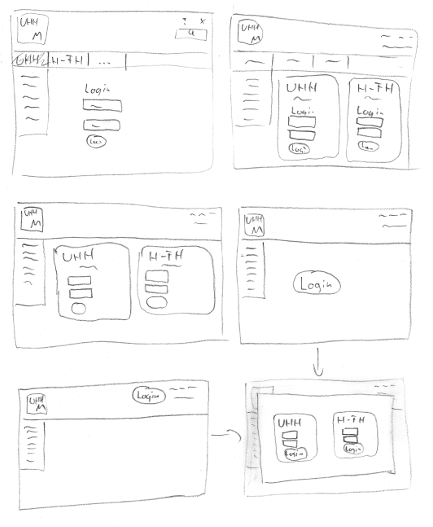
\includegraphics[width=1.0\textwidth]{Sketches-Login.png} 
	\caption{Sketches Login-Seite}
	\label{fig1}
\end{figure}
\begin{figure}[H]
	\centering
	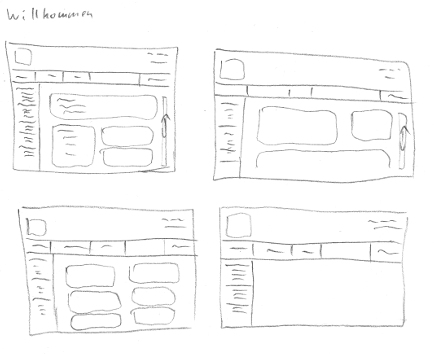
\includegraphics[width=1.0\textwidth]{Sketches-Willkommen.png} 
	\caption{Sketches Willkommen-Seite}
	\label{fig1}
\end{figure}



\item Implementierung

\begin{enumerate}
\item Login-Seite

Dem Menü auf der linken Seite wurde der Eintrag Login hinzugefügt. So kann man auf die Login-Seite zurückkehren, wenn man zuvor andere Menüpunkte angewählt hat.\\
Anstatt des Dropdown-Menüs zur Auswahl der Hochschule plus Login-Button wird ein einziger Login-Button benutzt, die Auswahl der Hochschule erfolgt später.\\
Die Aktivierung des Login-Buttons öffnet ein Popup-Panel. Dieses Fenster beinhaltet Anmelde-Pattern für beide Hochschulen. Der Benutzer kann sich jetzt bei der entsprechenden Hochschule anmelden. Danach schließt sich das Popup-Fenster wieder und die OLAT-Willkommen-Seite wird angezeigt. Die Seite mit geöffnetem Login-Popup kann auch direkt per Deep-linked State erreicht werden (vorher mußte man man auf der Hauptseite die Hochschule auswählen und konnte erst dann zur Login-Seite navigieren)\\\\
Das Popup-Panel wurde gewählt, um hervorzuheben, daß man sich nicht direkt an der OLAT-Seite anmeldet. Die Authentifizierung erfolgt stattdessen per Single-Sign-On auf einem anderen Server. Der Hilfe-Link leitet auf die Webseite des Anbieters weiter, der die Authentifizierung vornimmt (in diesem Falle das Rechenzentrum der UHH bzw. der Hamburger Fernhochschule).
\newpage
\begin{figure}[H]
	\centering
	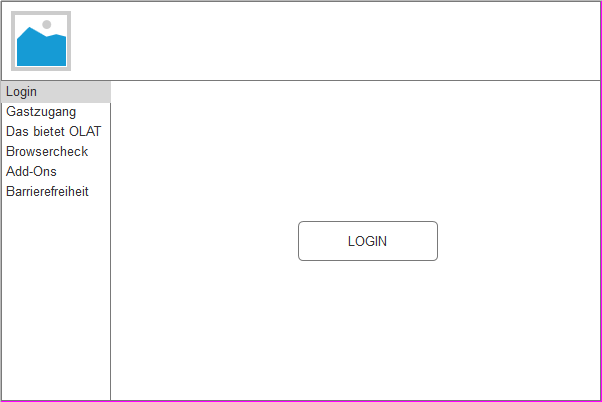
\includegraphics[width=1.0\textwidth]{Screenshot-Login.png} 
	\caption{Screenshot Login-Seite}
	\label{fig1}
\end{figure}
\begin{figure}[H]
	\centering
	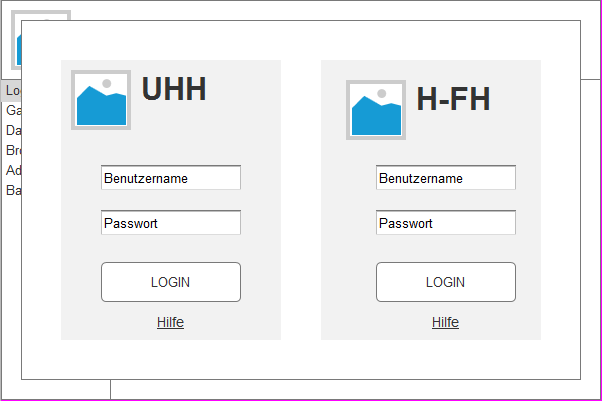
\includegraphics[width=1.0\textwidth]{Screenshot-Login-Popup.png} 
	\caption{Screenshot Login-Popup}
	\label{fig1}
\end{figure}

\newpage
\item Willkommen-Seite

Auch auf der Willkommen-Seite wurde das Corporate Design von OLAT/UHH beibehalten. Als 3. Menüebene wurde die Menüleiste am linken Rand durch Unterpunkte ergänzt, die die Tabs ersetzen, die auf der ursprünglichen Seite als 3. Menüebene z.B. Im Menüpunkt Einstellungen angezeigt wurden. Dadurch wird die Navigation übersichtlicher und man kann die Unterpunkte direkt anwählen.\\\\
Die Willkommen-Seite selbst enthält weiterhin ein konfigurierbares Dashboard.Der Konfigura- tions-Button wurde entfernt und ins Einstellungs-Menü verschoben. Darüber hinaus sind die Elemente des Dashboards besser konfigurierbar:  In der alten Version kann man nur einzelne Elemente (de-)aktivieren und ihre Position in einem 2 mal X-Grid festlegen. In der neuen Version kann man zusätzlich die Größe der Elemente einstellen.\\\\
Der Logout-Button (gehört zum UHH-Design und wurde daher hier nicht eingezeichnet) öffnet erneut ein Popup-Panel, mit dem man sich vom Authentifizierungs-Server abmelden kann. In der alten Version ist dieses nicht möglich, der Logout-Button hat keine Funktionalität, da man auch nach dem "Logout" am Authentifizierungs-Server angemeldet bleibt und durch erneutes Laden der OLAT-Seite wieder auf die Daten zugreifen kann.\\
Wenn man sich ausloggt, wird wieder die Login-Seite angezeigt.
\begin{figure}[H]
	\centering
	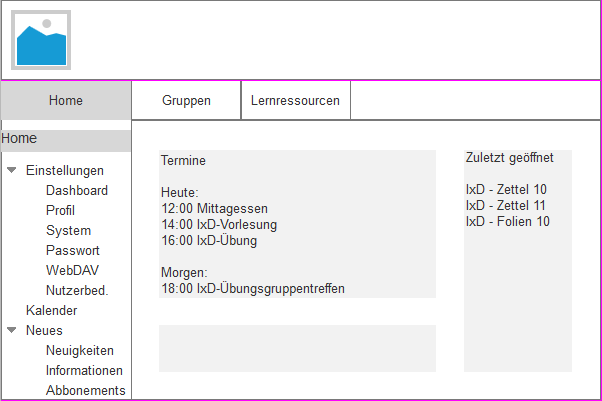
\includegraphics[width=1.0\textwidth]{Screenshot-Willkommen.png} 
	\caption{Screenshot Willkommen-Seite}
	\label{fig1}
\end{figure}
\begin{figure}[H]
	\centering
	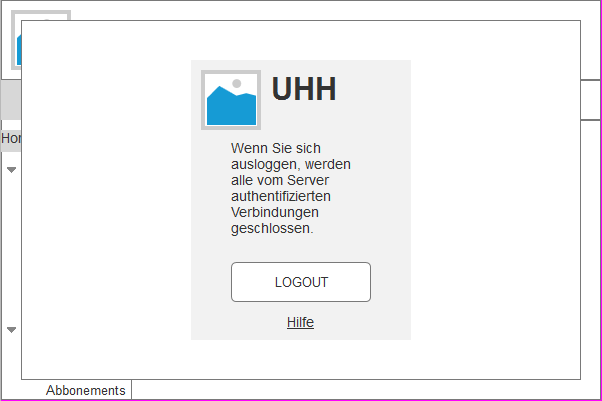
\includegraphics[width=1.0\textwidth]{Screenshot-Logout.png} 
	\caption{Screenshot Logout-Seite}
	\label{fig1}
\end{figure}
\end{enumerate}

\end{enumerate}
\end{document}
